\documentclass[12pt]{report}
    \title{\textbf{CAP4630 Intro to Artificial Intelligence \\ Knowledge-based
Intelligent System \\ Project 3 - Report}}
    \author{Tobias Dault, Eyob Tekle, William L. Thomson Jr.}
    \date{April 1st, 2022}

    \addtolength{\textheight}{3cm}
	\usepackage{enumitem}
    \usepackage{graphicx}
    \usepackage{hyperref}
    \usepackage[tmargin=1in,lmargin=1in,rmargin=1in]{geometry}
	\usepackage{titlesec}
    \graphicspath{ {./assets/} }

	\hypersetup{ colorlinks=true, linkcolor=blue, filecolor=purple, urlcolor=cyan }

    \newlength\tindent
    \setlength{\tindent}{\parindent}
    \setlength{\parindent}{0pt}
    \renewcommand{\indent}{\hspace*{\tindent}}

    \setlist[description]{noitemsep, topsep=0pt, itemsep=.5em}
    \setlist[enumerate]{noitemsep, topsep=0pt, itemsep=.5em}
    \setlist[itemize]{noitemsep, topsep=0pt, itemsep=.5em}

    \titleformat{\chapter}
	{\Large\bfseries}
	{\thechapter.}{0.5em}{}

	\titleformat{\section}
	{\large\bfseries}
	{\thesection.}{0.5em}{}

    \titlespacing\chapter{0pt}{12pt plus 0pt minus 4pt}{0pt plus 0pt minus 4pt}
    \titlespacing\section{0pt}{12pt plus 4pt minus 8pt}{0pt plus 2pt minus 8pt}

\begin{document}

\maketitle
\tableofcontents
\thispagestyle{empty}

\chapter{Overview}
\section{About}
This program is a knowledge-based intelligent system that collects user preferences and reasons about them. The program collects names of attributes, values of attributes ($A$), hard constraints represented as propositional formulas in conjunctive normal form (CNF) ($H$), and preferences languages of penalty logic, possibilistic logic, and qualitative choice logic with preference formulas ($T$) also in conjunctive normal form (CNF) from user input or files with the purpose of performing the following four reasoning tasks: \\

\begin{description}[style=multiline,leftmargin=12em]
  \item [Existence of Feasible Objects] Whether there are feasible objects w.r.t $H$,
that is, whether there are models of $H$ that are truth assignments making $H$ true.
  \item [Exemplification] Generate two random feasible objects, and show the preference between the two (strict preference or equivalence) w.r.t $T$
  \item [Optimization] Find an optimal object w.r.t $T$
  \item [Omni-Optimization] Find all optimal objects w.r.t $T$
\end{description}

\section{Design}
The program is written in Python and leverages the Tkinter python binding to TK GUI toolkit, used for the GUI of the program. The underlying logic is mostly performed with the use of clasp, an answer set solver for normal and disjunctive logic programs. The program wraps the clasp binary and uses it to perform tasks such as existence of feasible objects and for penalty and possibilistic preference logics. Qualitative choice logic is performed internally in the programs code without the use of clasp.


\chapter{Input}
Using a GUI written in Python (using Tkinter framework), input is taken through either the text input boxes or file input buttons.

\addtolength{\itemindent}{0.80cm}
\itemsep0em
\section{Binary Attributes}
Step 1: Follow steps in the README to start the program\\
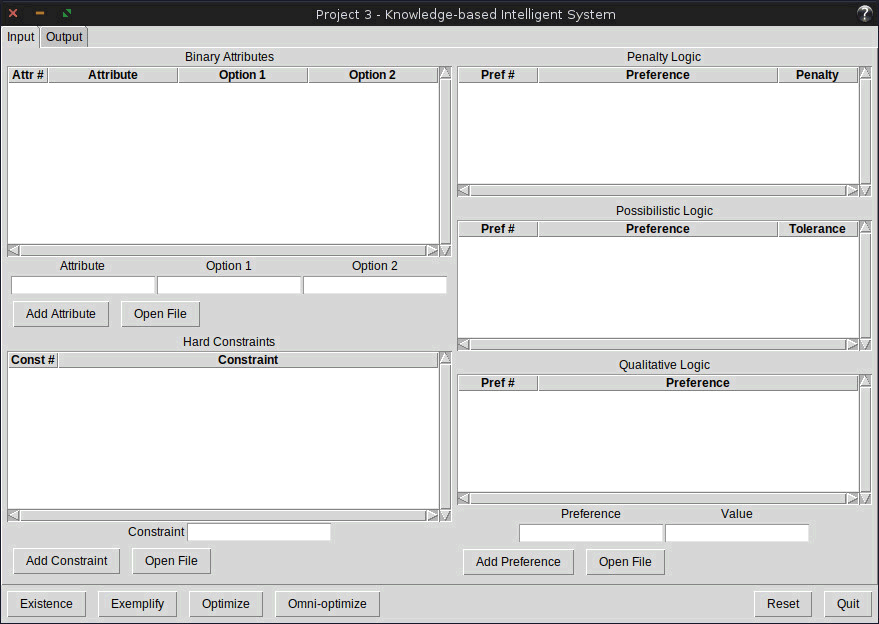
\includegraphics[scale=0.3]{input_start} \\\\
Step 2: Click the "Open File" button under Binary Attributes\\
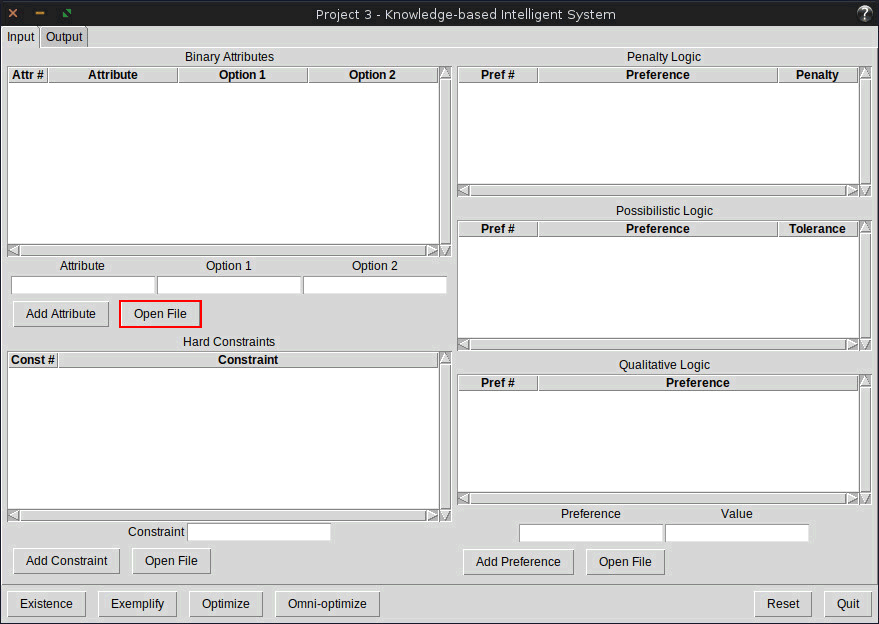
\includegraphics[scale=0.3]{input_attributes}\newpage
Step 3: Select your desired file (attributes$\_$test.txt for this example) and click "Open".\\
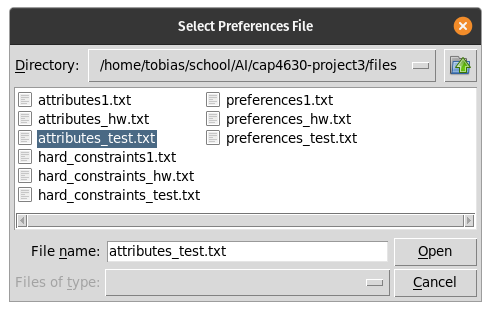
\includegraphics[scale=0.3]{select_attributes}\\
The contents of the file will be displayed under Binary Attributes.\\
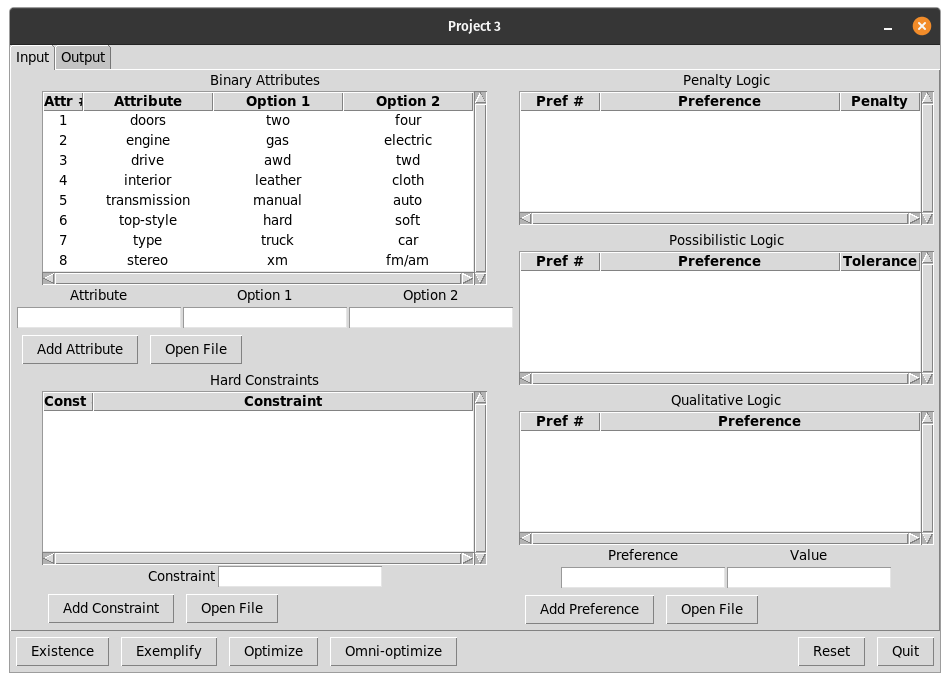
\includegraphics[scale=0.3]{attributes_imported}
\newpage

\section{Hard Constraints}
Step 1: Click the "Open File" button under Hard Constraints\\
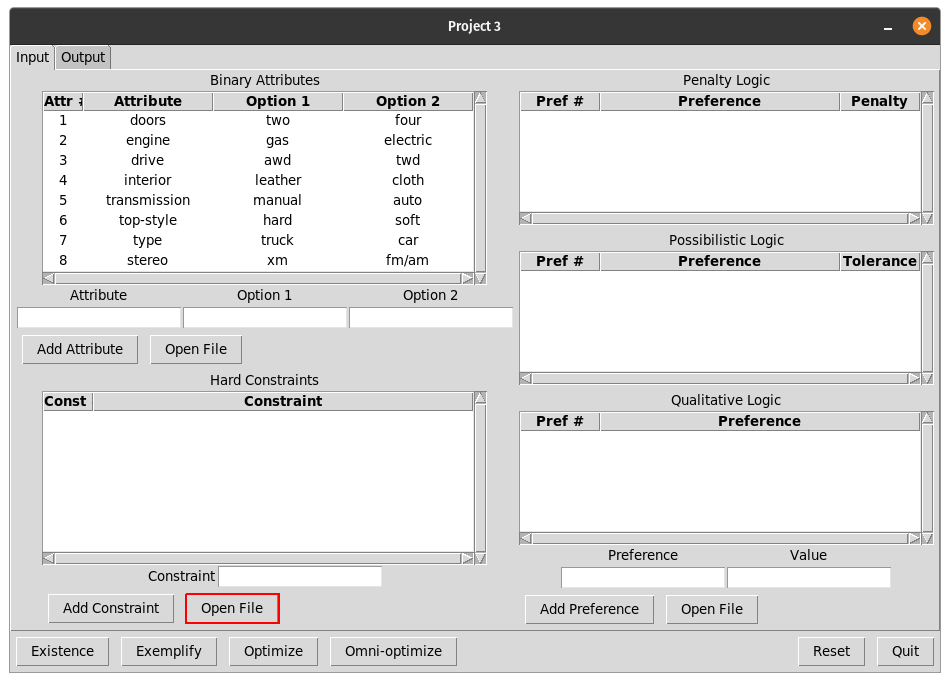
\includegraphics[scale=0.3]{input_constraints} \\\\
Step 2: Select your desired file (hard$\_$constraints$\_$test.txt for this example) and click "Open".\\
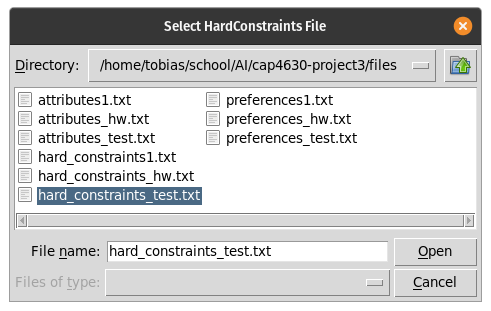
\includegraphics[scale=0.3]{select_constraints}\\
Step 3: The contents of the file will be displayed under Hard Constraints.\\
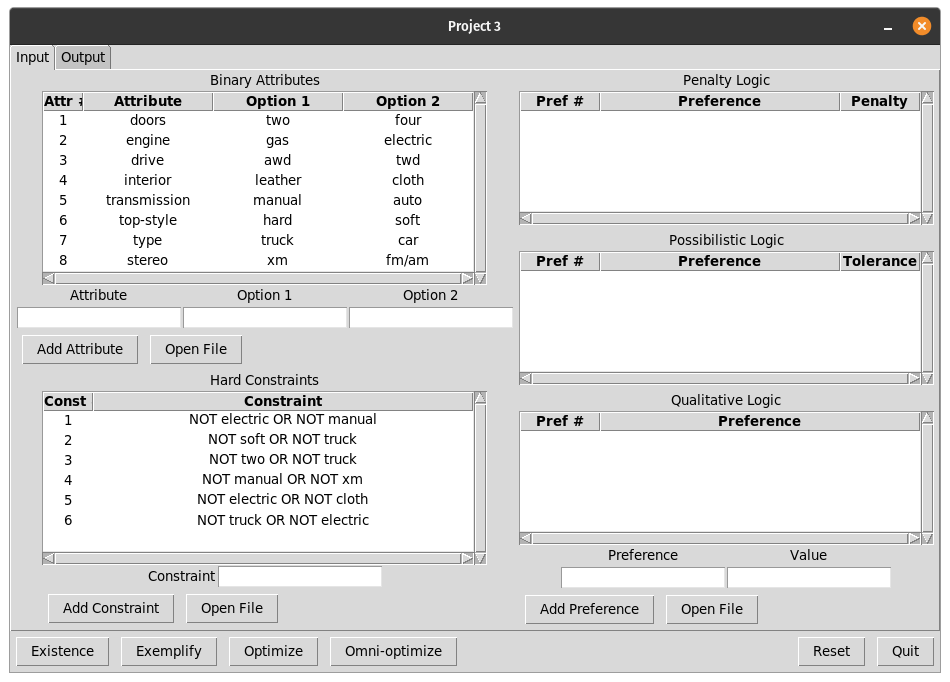
\includegraphics[scale=0.3]{constraints_imported}\\

\section{Logics}
Step 1: Click the "Open File" button under the three logics\\
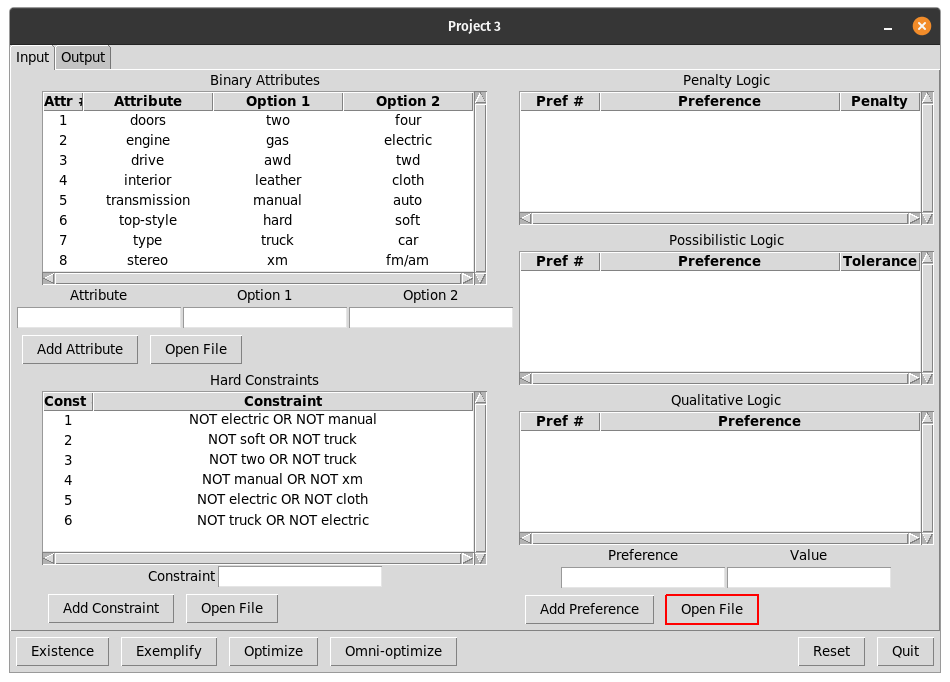
\includegraphics[scale=0.3]{input_preferences} \\\\
Step 2: Select your desired file (preferences$\_$test.txt for this example) and click "Open".\\
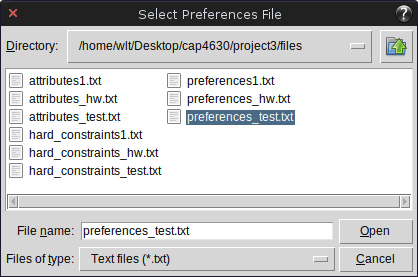
\includegraphics[scale=0.3]{select_preferences}\\
Step 3: The contents of the file will be displayed in the three.\\
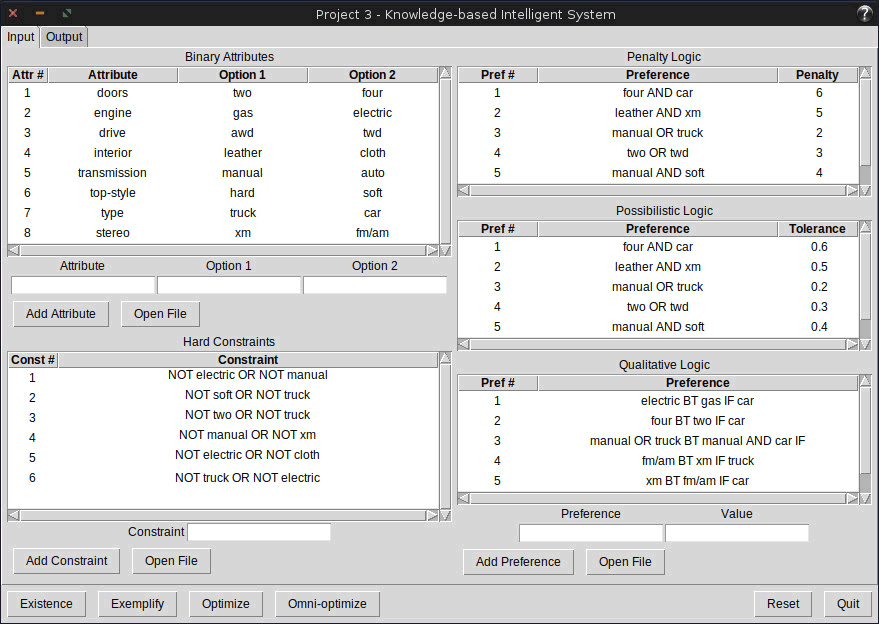
\includegraphics[scale=0.3]{preferences_imported}
\newpage

\chapter{Output}
\section{Existence of Feasible Objects} Click the "Existence" button\\
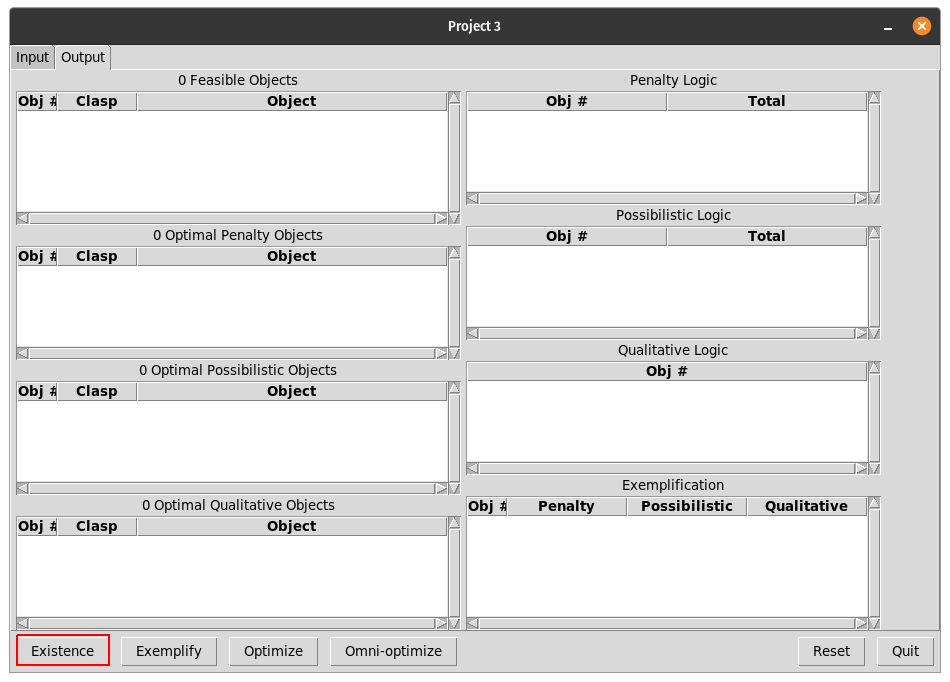
\includegraphics[scale=0.3]{existence}\\
All feasible objects, as well as a count of the total number of them, have been generated inside the "Feasible Objects" window.\\
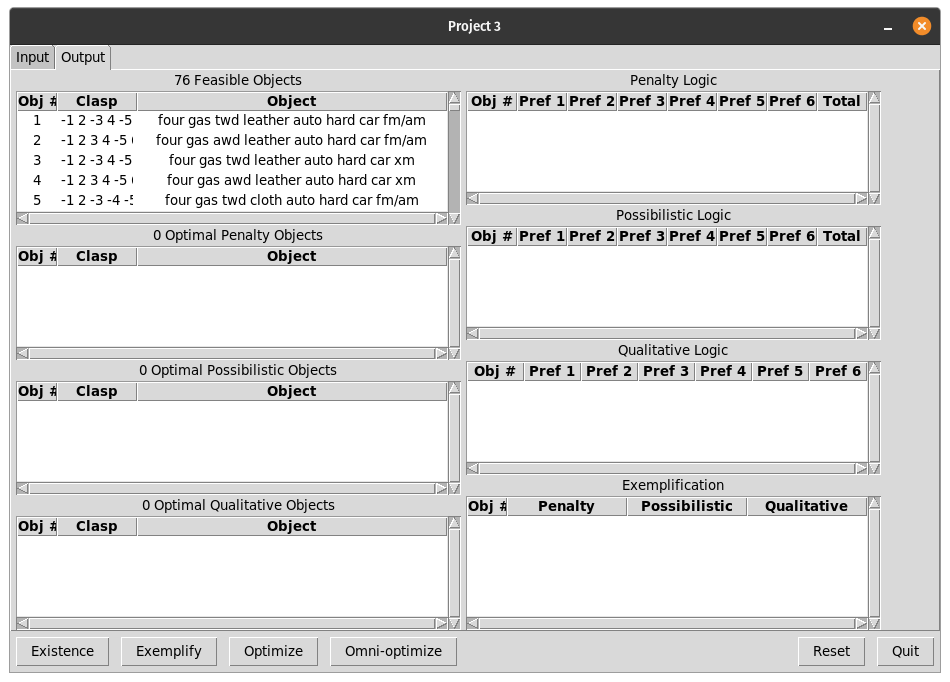
\includegraphics[scale=0.3]{post_existence}
\newpage

\section{Exemplify} Click the "Exemplify" button\\
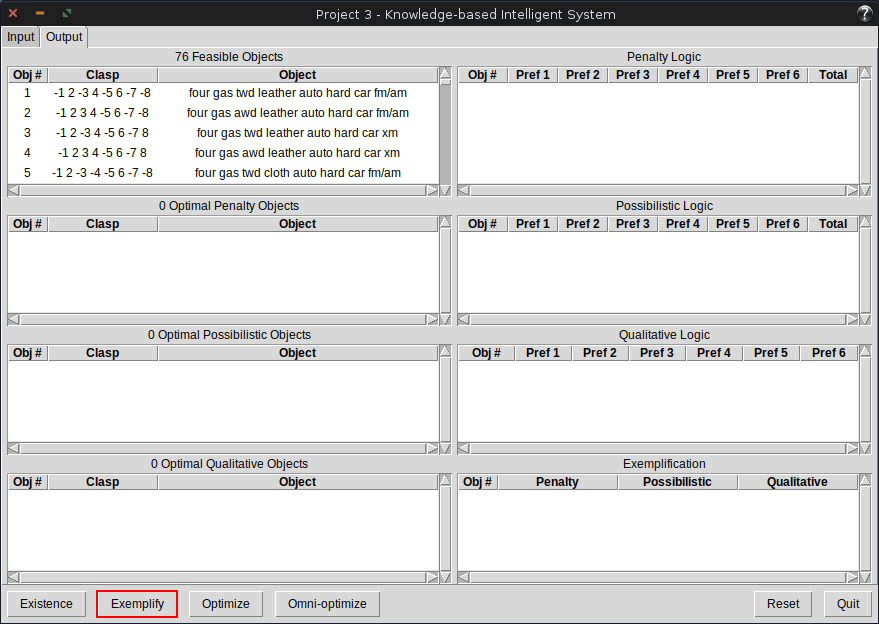
\includegraphics[scale=0.3]{exemplify}\\
The Penalty, Possiblistic, and Qualitative Logic tables have been generated. The exemplification table shows which objects are prefered for each logic.\\
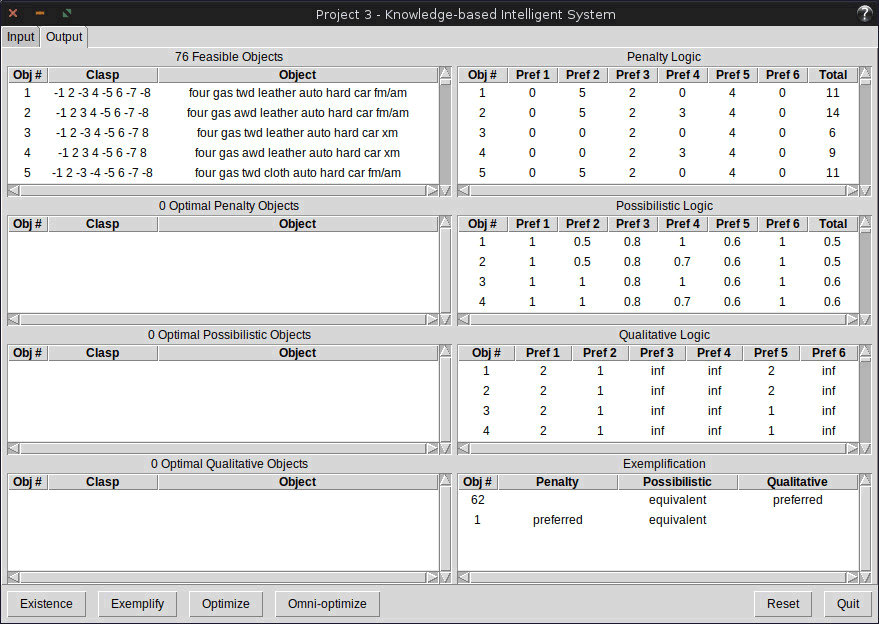
\includegraphics[scale=0.3]{post_exemplify}
\newpage

\section{Optimize} Click the "Optimize" button\\
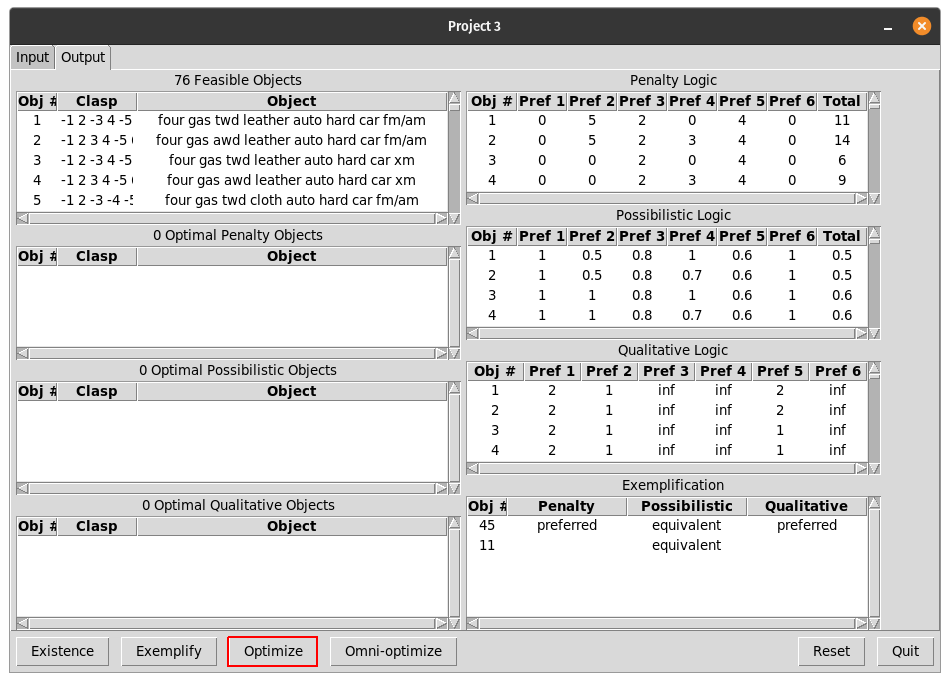
\includegraphics[scale=0.3]{optimize}\\
The Penalty, Possiblistic, and Qualitative Logic tables have been generated. The exemplification table shows which objects are prefered for each logic.\\
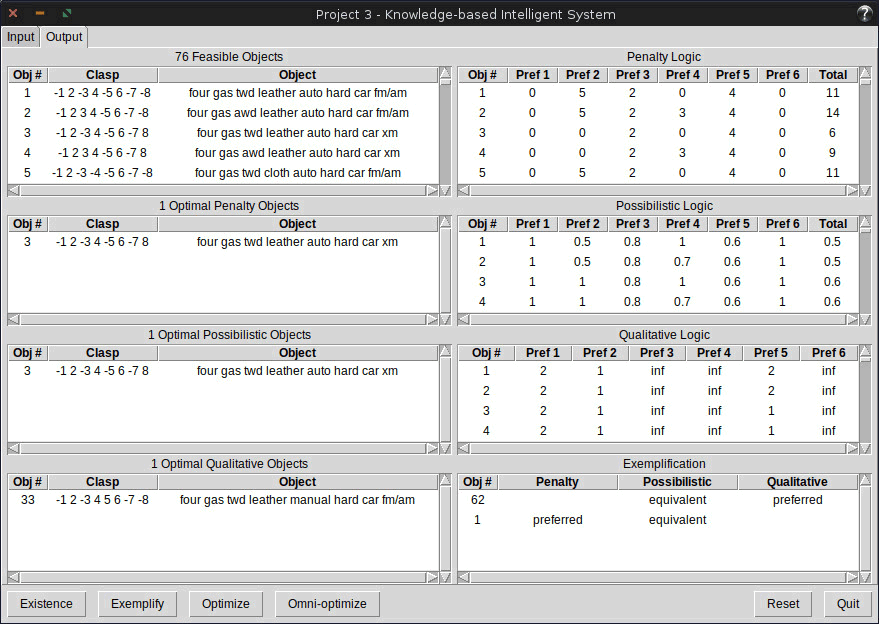
\includegraphics[scale=0.3]{post_optimize}
\newpage

\section{Omni-optimize} Click the "Omni-optimize" button\\
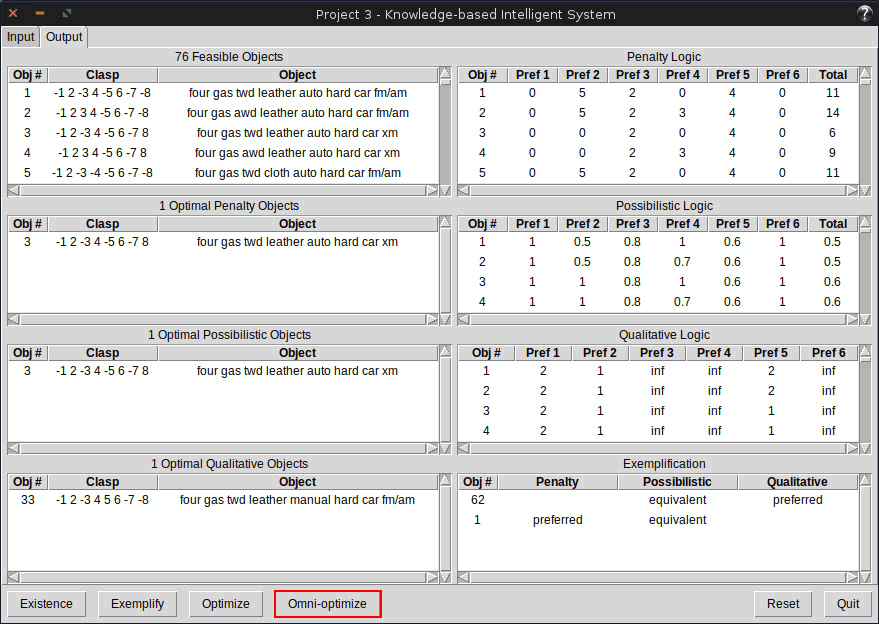
\includegraphics[scale=0.3]{omni-optimize}\\
The Penalty, Possiblistic, and Qualitative Logic tables have been generated. The exemplification table shows which objects are prefered for each logic.\\
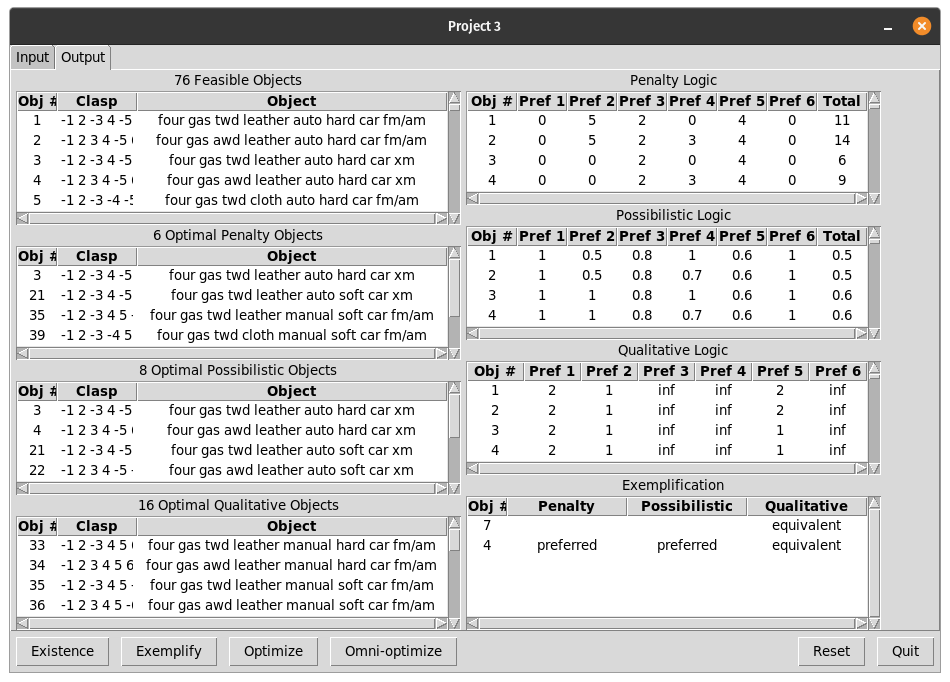
\includegraphics[scale=0.3]{post_omni-optimize}


\end{document}